
\section{Observations Information Model}
\label{sec:Observations Information Model}

The \gls{Observations Information Model} provides a representation of the data reported by a piece of equipment used for a manufacturing process, or used for any other purpose.  Additional descriptive information associated with the reported data is defined in the \block{MTConnectDevices} document, which is described in \citetitle{MTCPart2}.

Information defined in the \gls{Observations Information Model} allows a software application to (1) determine the value for \glspl{Data Entity} returned from a piece of equipment and (2) interpret the data associated with those \glspl{Data Entity} with the same meaning, value, and context that it had at its original source.  To do this, the software application issues one of two HTTP requests to an \gls{Agent} associated with a piece of equipment.  They are:


\begin{itemize}
\item \block{sample}:  Returns a designated number of time stamped \glspl{Data Entity} from an \gls{Agent} associated with a piece of equipment; subject to any HTTP filtering associated with the request.  See \textit{Section 8.3.3} of \citetitle{MTCPart1} of the MTConnect Standard for details on the \block{sample} HTTP request.

\item \block{current}:  Returns a snapshot of either the most recent values or the values at a given sequence number for all \glspl{Data Entity} associated with a piece of equipment from an \gls{Agent}; subject to any HTTP filtering associated with the request.  See \textit{Section 8.3.2} of \citetitle{MTCPart1} of the MTConnect Standard for details on the \block{current} HTTP request.
\end{itemize}

An \gls{Agent} responds to either the \block{sample} or \block{current} HTTP request with an \block{MTConnectStreams} \gls{Response Document}.  This document contains information describing \glspl{Data Entity} reported by an \gls{Agent} associated with a piece of equipment.   A client software application may correlate the information provided in the \block{MTConnectStreams} \gls{Response Document} with the physical and logical structure for that piece of equipment defined in the \block{MTConnectDevices} document to form a clear and unambiguous understanding of the information provided.  (See details on the structure for a piece of equipment described in \citetitle{MTCPart2}).

The \block{MTConnectStreams} \gls{Response Document} is comprised of two sections: \block{Header} and \block{Streams}.

The \block{Header} section contains protocol related information as defined in \textit{Section 6.5} of \citetitle{MTCPart1} of the MTConnect Standard.

The \block{Streams} section of the \block{MTConnectStreams} document contains a \block{DeviceStream} container for each piece of equipment represented in the document.  Each \block{DeviceStream} container is comprised of two primary types of elements – \glspl{Structural Element} and \glspl{Data Entity}.  The contents of the \block{DeviceStream} container are described in detail in this document, \citetitle{MTCPart3} of the MTConnect Standard.

\glspl{Structural Element} are defined for both the \block{MTConnectDevices} and the \block{MTConnectStreams} \glspl{Response Document}.  These \glspl{Structural Element} are used to provide a logical organization of the information provided in each document.  While used for a similar purpose, the \glspl{Structural Element} in the \block{MTConnectStreams} document are specifically designed to be distinctly different from those in the \block{MTConnectDevices} document:  

\begin{itemize}

\item \block{MTConnectDevices} document: \glspl{Structural Element} organize information that represents the physical and logical parts and sub-parts of a piece of equipment.  (See \citetitle{MTCPart2}, Section 4 of the MTConnect Standard for more details on \glspl{Structural Element} used in the \block{MTConnectDevices} document).  

\item \block{MTConnectStreams} document: \glspl{Structural Element} provide the structure to organize the data returned from a piece of equipment and establishes the proper context for that data.  The \glspl{Structural Element} specifically defined for use in the \block{MTConnectStreams} document are \block{DeviceStream} (see \sect{DeviceStream}) and \block{ComponentStream} (see \sect{ComponentStream}).   

\block{DeviceStream} and \block{ComponentStream} elements have a direct correlation to each of the \glspl{Structural Element} defined in the \block{MTConnectDevices} document.
\end{itemize}

\glspl{Data Entity} that describe data reported by a piece of equipment are also defined for both the \block{MTConnectDevices} and the \block{MTConnectStreams} \glspl{Response Document}.  The \glspl{Data Entity} provided in both documents directly relate to each other.  However, \glspl{Data Entity} are used for different purposes in each document:

\begin{itemize}
\item \block{MTConnectDevices} document: \gls{Data Entity} elements define the data that may be returned from a piece of equipment.  \citetitle{MTCPart2}, \textit{Sections 7 and 8} lists the possible \gls{Data Entity} elements that can be returned in a \block{MTConnectDevices} document.  

\item \block{MTConnectStreams} document: \gls{Data Entity} elements provide the data reported by a piece of equipment.  This data is organized in separate \block{ComponentStream} containers for each of the \glspl{Structural Element} defined in the \block{MTConnectDevices} document associated with the data that is reported by a piece of equipment.  
\end{itemize}

Within each \block{ComponentStream} container in the \block{MTConnectStreams} document, \glspl{Data Entity} are organized into three types of container elements - \block{Samples}, \block{Events}, and \block{Conditions}.  (See \sect{Observation Types} for more information on these elements.)

\section{Structural Elements for MTConnectStreams}
\label{sec:Structural Elements for MTConnectStreams}

\glspl{Structural Element} form the logical structure for the \gls{MTConnectStreams Response Document}.  These elements are used to organize the information and data that is reported by an \gls{Agent} for a piece of equipment.

\begin{figure}[ht]
  \centering
    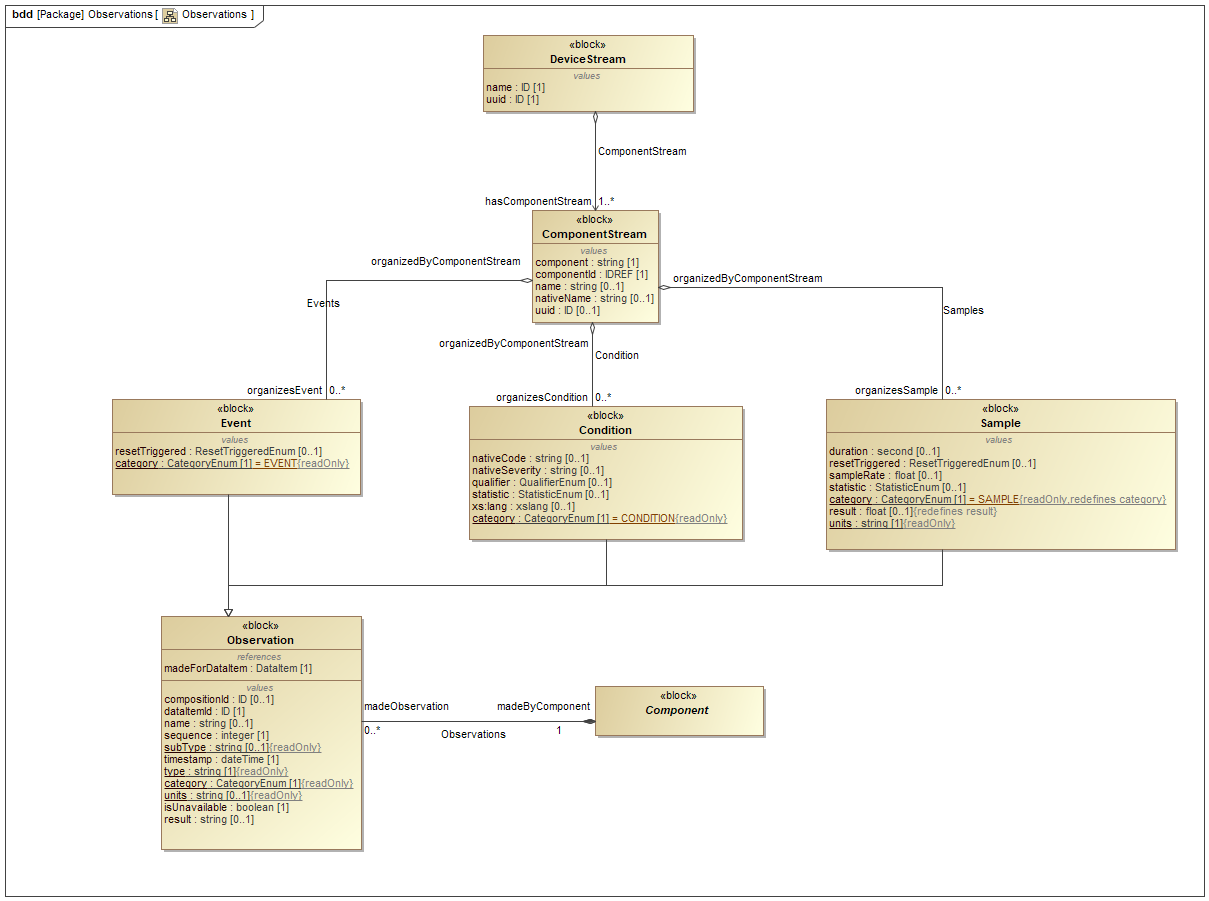
\includegraphics[width=1.0\textwidth]{figures/Observations.png}
  \caption{Observations Diagram}
  \label{fig:Observations Diagram}
\end{figure}

\FloatBarrier


Note: See \sect{Observations Schema Diagrams} for XML schema.

\input model-sections/Streams.tex

\input model-sections/Observations.tex

\input model-sections/Representation.tex

\section{Observation Types}
\label{sec:Observation Types}

\block{Observation} elements are represented by \block{Sample}, \block{Event} or \block{Condition} elements based upon the \property{category} and \property{type} attributes defined for the corresponding \block{DataItem}.

\input model-sections/ConditionStates.tex

\input model-sections/ConditionTypes.tex

\input model-sections/EventTypes.tex

\input model-sections/SampleTypes.tex
